\chapter{Introduction to Data Visualization in Python (Matplotlib and Seaborn)}

\section{Introduction: Real-Life Hook}

Think about situations in student life:

\begin{itemize}
    \item You track your exam scores over the year  
    \item You compare marks in different subjects  
    \item You visualize sports scores or attendance trends  
\end{itemize}

\textbf{Charts and graphs} make it easier to understand patterns. Python provides \textbf{Matplotlib} and \textbf{Seaborn} for data visualization.

\section{Concept: Why Visualize Data?}

\begin{definition}{Data Visualization}
Data visualization is the process of \textbf{representing data graphically} to make patterns, trends, and insights easier to understand.
\end{definition}

Benefits:

\begin{itemize}
    \item Makes complex data \textbf{easy to understand}  
    \item Helps \textbf{compare and analyze} trends  
    \item Makes reports and presentations \textbf{attractive}  
\end{itemize}

\section{Getting Started with Matplotlib}

Install if needed:

\begin{verbatim}
pip install matplotlib
\end{verbatim}

\subsection{Example: Line Chart of Exam Scores}

\begin{verbatim}
import matplotlib.pyplot as plt

subjects = ["Math", "Science", "English", "History"]
marks = [85, 90, 78, 88]

plt.plot(subjects, marks, marker='o', color='blue', linestyle='-')
plt.title("Exam Scores")
plt.xlabel("Subjects")
plt.ylabel("Marks")
plt.grid(True)
plt.show()
\end{verbatim}

- \texttt{plt.plot()} draws a line chart  
- \texttt{marker} adds points, \texttt{linestyle} adds line style  
- \texttt{plt.show()} displays the chart  

\subsection{Bar Chart Example}

\begin{verbatim}
plt.bar(subjects, marks, color='green')
plt.title("Exam Scores Bar Chart")
plt.xlabel("Subjects")
plt.ylabel("Marks")
plt.show()
\end{verbatim}

\subsection{Histogram Example}

\begin{verbatim}
marks = [85, 90, 78, 88, 92, 76, 84]
plt.hist(marks, bins=5, color='orange')
plt.title("Marks Distribution")
plt.xlabel("Marks Range")
plt.ylabel("Number of Students")
plt.show()
\end{verbatim}

\section{Introduction to Seaborn}

Seaborn makes \textbf{beautiful statistical charts}:

Install:

\begin{verbatim}
pip install seaborn
\end{verbatim}

\subsection{Example: Seaborn Bar Plot}

\begin{verbatim}
import seaborn as sns
import matplotlib.pyplot as plt

data = {"Subjects": ["Math", "Science", "English", "History"],
        "Marks": [85, 90, 78, 88]}

sns.barplot(x="Subjects", y="Marks", data=data)
plt.title("Seaborn Bar Chart")
plt.show()
\end{verbatim}

- Seaborn integrates with \textbf{Pandas} and Matplotlib  
- Adds \textbf{color palettes and styles} easily  

\section{Mini-Project: Visualizing Student Performance}

\begin{verbatim}
import matplotlib.pyplot as plt
import seaborn as sns

# Data
students = ["Amina", "Rafi", "Nabil", "Sara"]
math = [85, 78, 92, 88]
science = [90, 80, 85, 91]

# Line plot with Matplotlib
plt.plot(students, math, marker='o', label='Math')
plt.plot(students, science, marker='s', label='Science')
plt.title("Student Marks Line Chart")
plt.xlabel("Students")
plt.ylabel("Marks")
plt.legend()
plt.show()

# Bar plot with Seaborn
import pandas as pd
df = pd.DataFrame({
    "Student": students*2,
    "Subject": ["Math"]*4 + ["Science"]*4,
    "Marks": math + science
})

sns.barplot(x="Student", y="Marks", hue="Subject", data=df)
plt.title("Student Marks Comparison")
plt.show()
\end{verbatim}

- Students learn \textbf{line charts, bar charts, multiple data comparison}  

\section{Step-by-Step Diagram: Data Visualization Workflow}

\begin{center}
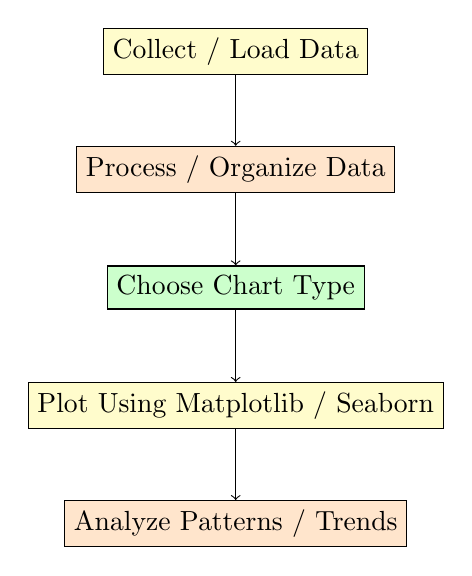
\begin{tikzpicture}[node distance=1.5cm]
\node (data) [draw, rectangle, fill=yellow!20] {Collect / Load Data};
\node (process) [draw, rectangle, fill=orange!20, below of=data] {Process / Organize Data};
\node (choose) [draw, rectangle, fill=green!20, below of=process] {Choose Chart Type};
\node (visualize) [draw, rectangle, fill=yellow!20, below of=choose] {Plot Using Matplotlib / Seaborn};
\node (analyze) [draw, rectangle, fill=orange!20, below of=visualize] {Analyze Patterns / Trends};
\draw[->] (data) -- (process);
\draw[->] (process) -- (choose);
\draw[->] (choose) -- (visualize);
\draw[->] (visualize) -- (analyze);
\end{tikzpicture}
\end{center}

\section{Key Concepts}

\begin{itemize}
    \item Data visualization converts raw data into visual charts  
    \item \textbf{Matplotlib}: basic charts, highly customizable  
    \item \textbf{Seaborn}: advanced statistical charts, easier and prettier  
    \item Charts include line, bar, histogram, scatter, and more  
    \item Visualization helps identify trends and compare data  
\end{itemize}

\section{End-of-Chapter Exercises}

\begin{exercise}{Very Short Questions}
\begin{enumerate}
    \item Name two Python libraries used for data visualization.  
    \item What is the purpose of data visualization?  
    \item Name three types of charts.  
\end{enumerate}
\end{exercise}

\begin{exercise}{Short Answer Questions}
\begin{enumerate}
    \item Create a line chart showing the marks of 5 students in one subject.  
    \item Create a bar chart comparing marks in two subjects for 4 students.  
    \item Explain the difference between Matplotlib and Seaborn.  
\end{enumerate}
\end{exercise}

\begin{exercise}{Activity-Based Questions}
\begin{enumerate}
    \item Collect the scores of your class in Math, Science, and English. Create a line chart for each subject.  
    \item Create a histogram showing the distribution of students’ scores.  
    \item Use Seaborn to create a bar chart comparing the average marks of boys vs girls in your class.  
\end{enumerate}
\end{exercise}

\section{Teacher Notes}

\marginnote{
\textbf{Learning Objectives:}  
\begin{itemize}
    \item Students can create line, bar, and histogram charts  
    \item Students understand chart types and when to use them  
    \item Students can visualize data using Matplotlib and Seaborn  
\end{itemize}

\textbf{Teaching Tips:}  
\begin{itemize}
    \item Start with simple datasets (like student marks)  
    \item Demonstrate Matplotlib first, then Seaborn for advanced visuals  
    \item Encourage students to explore colors, styles, and labels  
\end{itemize}

\textbf{Assessment:}  
\begin{itemize}
    \item Check correctness of charts and labels  
    \item Observe ability to compare and interpret data visually  
\end{itemize}
}